\documentclass{beamer}
%Information to be included in the title page:

\usepackage{amsmath, mathtools, tikz}
\usetikzlibrary{calc, positioning, cd}
\usetikzlibrary{arrows.meta}

\uselanguage{italian}
\languagepath{italian}
\deftranslation[to=italian]{Definition}{Definizione}
\deftranslation[to=italian]{Theorem}{Teorema}
\deftranslation[to=italian]{Proposition}{Proposizione}

\deftranslation[to=italian]{Example}{Esempio}

\newenvironment{exercise}[1][]
{
  \begin{exampleblock}{Esercizio #1}
}
{
  \end{exampleblock}
}



\AtBeginSection[]{
  \begin{frame}
    \frametitle{Outline}
    \tableofcontents[currentsection]
  \end{frame}
}



\newcommand{\Hom}{\mathrm{Hom}}
\newcommand{\im}{\mathrm{im}\,}
\newcommand{\obj}{\mathrm{obj}}
\newcommand{\Vertk}{\mathrm{Vert}}
\newcommand{\Dr}[1]{\ensuremath{\underset{#1}{\textnormal{Dr}}}}

\newcommand{\ssedef}{\mathrel{\stackrel{\mathrm{def}}{\Leftrightarrow}}}

\newcommand{\cat}[1]{\mathrm{\mathbf{#1}}}

\usetheme{Warsaw}
\usefonttheme[onlymath]{serif}

\addtobeamertemplate{navigation symbols}{}{%
    \usebeamerfont{footline}%
    \usebeamercolor[fg]{footline}%
    \hspace{1em}%
    \insertframenumber/\inserttotalframenumber
}

\title{Coomologia di Čech}
\author{Dario Di Meo (D70/000023)}
\date{Seminario di Geometria Algebrica, a.a. 2025/2026}

\begin{document}

\frame{\titlepage}

\section{Coomologia di Čech}

\subsection{Coomologia di un ricoprimento a coefficienti in un fascio}

\begin{frame}
    \begin{definition}[Complesso simpliciale astratto]
        \pause
    Un complesso simpliciale astratto $K$ è una coppia
    $$K=\left(\Vertk(K),\Sigma\right)$$
    dove
    \pause
    \begin{enumerate}
        \item $\Vertk(K)$ è un inieme non vuoto di elementi chiamati \textbf{vertici};
        \pause
        \item $\Sigma$ è un sottoinsieme di parti finite e non vuote di $\Vertk(K)$ chiamate \textbf{simplessi} tali che
        \pause
        \begin{enumerate}[(i.)]
            \item Per ogni $v\in\Vertk(K)$, $\{v\}\in\Sigma$;
            \pause
            \item $\sigma\in\Sigma\wedge\emptyset\ne\tau\subseteq\sigma\Rightarrow\tau\in\Sigma$.
        \end{enumerate}
    \end{enumerate}
    \end{definition}
    \pause
    Se $\sigma$ è un simplesso e $|\sigma|=q+1$, $\sigma$ si dirà $q$-simplesso.
    \pause

    Il sottoinsieme di $\Sigma$ di tutti i $q$-simplessi si indicherà con $\Sigma_q$.
\end{frame}

\begin{frame}
    Si fissi uno spazio topologico $X$.

    \begin{definition}[Nervo]
        \pause
        Sia $\mathcal{U}$ un ricoprimento aperto di $X$. \pause
        
        Si dice \textbf{nervo}, e si indica con $N(\mathcal{U})$, il complesso simpliciale astratto i cui vertici sono gli aperti del ricoprimento, vale a dire $\Vertk(N(\mathcal{U}))=\mathcal{U}$, \pause e i cui simplessi sono le sottofamiglie finite di $\mathcal{U}$ a intersezione non vuota:
    $$\mathcal{S}=\Bigg\{(U_{i_0},U_{i_1},...,U_{i_n}):n\in\mathbb{N}_0\wedge\bigcap_{j=0}^nU_{i_j}\ne\emptyset\Bigg\}$$
    \end{definition}
\end{frame}

\begin{frame}
    \begin{definition}[Complesso di gruppi di cocatene]
        \pause
        Definiamo la seguente successione di gruppi e omomorfismi
        $$C^\bullet(N(\mathcal{U}),\mathcal{F})=\cdots\longrightarrow C^q(\mathcal{U},\mathcal{F})\xrightarrow{\delta^q}C^{q+1}(\mathcal{U},\mathcal{F})\longrightarrow\cdots$$
        dove:
        \pause
        $C^q(\mathcal{U},\mathcal{F})= \Dr{\sigma\in\Sigma_q}\mathcal{F}\left(\bigcap \sigma\right)$
        \pause
        e, presa $f:\Sigma_q\rightarrow\bigcup_{\sigma\in\Sigma_q}\mathcal{F}\left(\bigcap\sigma\right)$ in $C^q(\mathcal{U},\mathcal{F})$:
        
        $$\delta^q(f)=\left(\sigma\in\Sigma_{q+1}\mapsto\sum_{i=0}^{q+1}(-1)^i f\left(\hat{\sigma}^i\right)\in\bigcup_{\sigma\in\Sigma_{q+1}}\mathcal{F}\left(\bigcap\sigma\right)\right)$$
    
        in $C^{q+1}(\mathcal{F},\mathcal{U})$.
    \end{definition}
\end{frame}

\begin{frame}
    \begin{exercise}
        \pause
        $$\boxed{C^\bullet(N(\mathcal{U}),\mathcal{F})\textnormal{ è un complesso.}}$$
    \end{exercise}
    \pause

\begin{definition}[Coomologia di un ricoprimento a coefficienti in $\mathcal{F}$]
    \pause
    Siano $\mathcal{U}$ un ricoprimento aperto di $X$ e $\mathcal{F}$ un fascio di gruppi abeliani su $X$.
    \pause

    Chiamiamo \textbf{gruppi di coomologia} di $\mathcal{U}$ con coefficienti in $\mathcal{F}$, e li indichiamo con
    $$\check{H}^q(\mathcal{U},\mathcal{F})$$
    i gruppi di omologia del complesso $C^\bullet(N(\mathcal{U}),\mathcal{F})$.
\end{definition}

\end{frame}

\subsection{Limiti diretti}

\begin{frame}
    \begin{definition}[Sistema diretto]
        \pause
        Siano $(I,\preceq)$ un insieme parzialmente ordinato e $\mathcal{C}$ una categoria. 
        \pause
        
        Un \textbf{sistema diretto} in $\mathcal{C}$ su $I$ è una coppia ordinata
        $$\{M_i,\varphi^i_j\}\coloneq\left((M_i)_{i\in I},(\varphi^i_j)_{i\preceq j}\right)$$
        dove \pause $(M_i)_{i\in I}\subseteq\obj(\mathcal{C})$; \pause $(\varphi^i_j)_{i\preceq j}\subseteq {M_j}^{M_i}$ con $\varphi^i_i=\iota_{M_i}$ per ogni $i$; \pause per ogni $i\preceq j\preceq k$, il seguente diagramma è commutativo:
        \[
        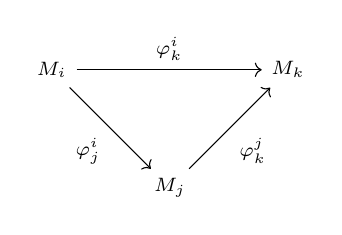
\begin{tikzpicture}[->, node distance=1.5cm, font=\scriptsize]
        \node (Mi) {$M_i$};
        \node (A) [right of=Mi] {};
        \node (Mk) [right of=A] {$M_k$};
        \node (Mj) [below of=A] {$M_j$};

        \draw (Mi) -- (Mk) node[midway, above] {$\varphi^i_k$};
        \draw (Mi) -- (Mj) node[midway, below left] {$\varphi^i_j$};
        \draw (Mj) -- (Mk) node[midway, below right] {$\varphi^j_k$};

        \end{tikzpicture}
        \]
    \end{definition}
\end{frame}

\begin{frame}
    
    \begin{definition}[Limite diretto] % insertion morfisms
        \pause
        Siano $(I,\preceq)$ un poset, $\mathcal{C}$ una categoria e $\{M_i,\varphi^i_j\}$ diretto in $\mathcal{C}$. 
        \pause
        
        Il \textbf{limite diretto} è una coppia costituita da un oggetto $\varinjlim M_i$ e da una famiglia $(\alpha_i)_{i\in I}\subseteq (\varinjlim M_i)^{M_i}$ di \textbf{insertion morfisms} tali che
        \begin{enumerate}[i]
            \pause
            \item $\varphi^i_j\cdot\alpha_j=\alpha_i$ quando $i\preceq j$;
            \pause
            \item Presi $X\in\obj(\mathcal{C})$ e dei morfismi $f_i:M_i\rightarrow X$ t.c. $\varphi^i_j\cdot f_j=f_i$ per ogni $i\preceq j$, esiste ed è unico $\theta:\varinjlim M_i\rightarrow X$ che rende il seguente diagramma commutativo:
            \vspace{-0.4cm}
            \[
            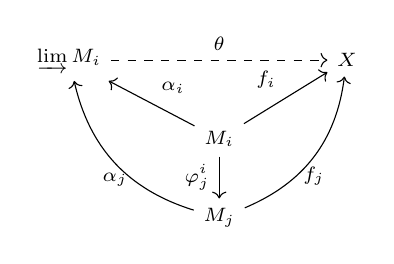
\begin{tikzpicture}[->, node distance=1cm, font=\scriptsize]
            \node (lim) {$\varinjlim M_i$};
            \node (A) [right=1.25cm of lim] {};
            \node (X) [right=1.25cm of A] {$X$};
            \node (Mi) [below of=A] {$M_i$};
            \node (Mj) [below of=Mi] {$M_j$};

            \draw[dashed] (lim) -- (X) node[midway, above] {$\theta$};
            \draw (Mi) -- (lim) node[midway, above right] {$\alpha_i$};
            \draw (Mi) -- (X) node[midway, above left] {$f_i$};
            \draw (Mi) -- (Mj) node[midway, left] {$\varphi^i_j$};
            \draw (Mj) to[bend left] node[midway, below] {$\alpha_j$} (lim);
            \draw (Mj) to[bend right] node[midway, below] {$f_j$} (X);

            \end{tikzpicture}
            \]
        \end{enumerate}        
    \end{definition}
\end{frame}

\begin{frame}
    \begin{definition}[Classe diretta]
        \pause
        Una classe $\mathcal{K}$ si dice \textbf{classe diretta} se su di essa è definita una relazione $\preceq$ riflessiva, asimmetrica e transitiva e se per ogni $k,k'\in\mathcal{K}$ esiste $k^*\in\mathcal{K}$ tale che $k\preceq k^*$ e $k'\preceq k^*$.
    \end{definition}
\pause
    \begin{definition}[Sottoclasse cofinale]
        \pause
        Una sottoclasse $\mathcal{L}$ di $\mathcal{K}$ si dice \textbf{cofinale} in $\mathcal{K}$ se, per ogni $k\in\mathcal{K}$, esiste $l\in\mathcal{L}$ tale che $k\preceq l$.
    \end{definition}
\pause
    È possibile definire i sistemi diretti anche a partire da una classe diretta.
\end{frame}

\begin{frame} % Una categoria è cocompleta se per ogni sistema diretto esiste il colimite
    \begin{definition}[Categoria cocompleta]
        \pause
        Una categoria $\mathcal{C}$ si dice \textbf{cocompleta} se il limite diretto esiste per ogni sistema diretto in $\mathcal{C}$.
    \end{definition}
    \pause
    \begin{block}{Proposizione}
    \pause
    Siano $\mathcal{K}$ una classe diretta, $\mathcal{C}$ una categoria cocompleta e $\{A_k,\varphi^k_j\}$ un sistema diretto in $\mathcal{C}$ su $\mathcal{K}$. \pause Se due sottoclassi di $\mathcal{K}$, siano esse $\mathcal{L}$ e $\mathcal{M}$, sono insiemi e cofinali in $\mathcal{K}$, allora
    $$\boxed{\varinjlim\nolimits_\mathcal{L}A_k\cong\varinjlim\nolimits_\mathcal{M}A_k}$$
    \end{block}
\end{frame}

\subsection{Coomologia di Čech}

\begin{frame}
    \begin{definition}[Raffinamento]
        \pause
        Siano $\mathcal{U}$ e $\mathcal{V}$ due ricoprimenti aperti di $X$.
        \pause

        $\mathcal{V}$ si dice \textbf{raffinamento} di $\mathcal{U}$, e si indica con $\mathcal{U}\preceq\mathcal{V}$, se, per ogni $V\in\mathcal{V}$, esiste $U\in\mathcal{U}$ tale che $V\subseteq U$.
    \end{definition}
    \pause
    \begin{definition}[Funzione di raffinamento]
        \pause
        Siano $\mathcal{U}$ e $\mathcal{V}$ due ricoprimenti aperti di $X$ tali che $\mathcal{U}\preceq\mathcal{V}$.
        \pause

        Scegliere, al variare di $V\in\mathcal{V}$, $V\subseteq U_V\in\mathcal{U}$ definisce una funzione
        $$r:V\in\mathcal{V}\mapsto U_V\in\mathcal{U}$$
        detta \textbf{funzione di raffinamento}.
    \end{definition}
\end{frame}

\begin{frame}
    \begin{definition}[Ordine parziale sugli $\check{H}^q(\mathcal{U},\mathcal{F})$]
        \pause
        Sia $\mathcal{F}$ un fascio di gruppi abeliani su $X$.
        \pause
        
        Poniamo $\check{H}^q(\mathcal{U},\mathcal{F})\preceq\check{H}^q(\mathcal{V},\mathcal{F})$ se e solo se, per definizione, esiste una funzione di raffinamento $r:\mathcal{V}\rightarrow\mathcal{U}$.
        \pause

        (Si dimosta che) $\preceq$ è un ordine parziale sugli $\check{H}^q(\mathcal{U},\mathcal{F})$.
    \end{definition}
\end{frame}

\begin{frame}
    \begin{exercise}[(Ricerca di un sottoinsieme cofinale in $\mathcal{K}$)]
        \pause
        Sia $\mathcal{K}$ la classe diretta dei gruppi $\check{H}^q(\mathcal{U},\mathcal{F})$.
        \pause
        \[
        \boxed{
        \begin{aligned}
             &\textnormal{La sottoclasse} \\
             &\mathcal{H}\coloneq\{\check{H}^q(\mathcal{U},\mathcal{F}):\mathcal{U}\textnormal{ è un ricoprimento aperto senza ripetizioni}\} \\\
        &\textnormal{è un insieme cofinale in }\mathcal{K}.   
        \end{aligned}    
        }
        \]

 
    \end{exercise}
    \pause
    \begin{definition}[Comologia di Čech]
        \pause
        La \textbf{coomologia di Čech di $X$ a coefficienti nel fascio $\mathcal{F}$ su $X$} è definita come 
        $$\check{H}^q(X,\mathcal{F})\coloneq\varinjlim\nolimits_\mathcal{H}\check{H}^q(\mathcal{U,\mathcal{F}})$$
    \end{definition}
\end{frame}

\section{Confronto tra le coomologie}


\begin{frame}
    \begin{exercise}[(Coomologia di Čech di grado 0)]
        $$\boxed{\check{H}^0(X,\mathcal{U})=\Gamma(\mathcal{F})=\mathcal{F}(X)}$$
    \end{exercise}
\end{frame}


%\begin{frame}
%    Noi vogliamo usare questa per dire che le due coomologie so' uguali:
%    \begin{block}{Proposizione}
%        Siano $(F^n)_{n\in\mathbb{N}_0}$ e $(F'^n)_{n\in\mathbb{N}_0}$ due successioni di funtori covarianti additivi tra categorie abeliane $\mathcal{A}$ e $\mathcal{B}$ dove $\mathcal{A}$ ha abbastanza iniettivi. SUpponiamo che 
%        \begin{enumerate}[(i)]
%            \item Per ogni successione esatta corta, c'è una successione esatta lunga con natural connecting homomorphisms;
%            \item $F^0$ è naturalmente isomorfo a $F'^0$;
%            \item $F^n(E)=0=F'^n(E)$ per tutti gli oggetti iniettivi $E$ e per ogni $n\geq 1$. 
%        \end{enumerate} 
%        Allora $F^n$ è naturalmente isomorfo a $F'^n$ per ogni $n\in\mathbb{N}_0$.
%    \end{block}
%\end{frame}

\begin{frame}
    Noi vogliamo usare questa per dire che le due coomologie so' uguali:
    \begin{block}{Proposizione}
        Siano $(F^n)_{n\in\mathbb{N}_0}$ e $(G^n)_{n\in\mathbb{N}_0}$ due successioni di funtori covarianti additivi tali che $F^n,G^n:\mathrm{\mathbf{Sh}}(X,\mathrm{\mathbf{Ab}})\rightarrow\mathrm{\mathbf{Ab}}$ per ogni $n\in\mathbb{N}_0$. Supponiamo che
        \begin{enumerate}[(i)]
            \item Per ogni successione esatta corta, c'è una successione esatta lunga con natural connecting homomorphisms;
            \item $F^0$ è naturalmente isomorfo a $F'^0$;
            \item $F^n(E)=0=F'^n(E)$ per tutti gli oggetti iniettivi $E$ e per ogni $n\geq 1$. 
        \end{enumerate} 
    \end{block}
\end{frame}

\begin{frame}
    Questo appara il punto 1:
    \begin{theorem}[Serre]
        Se $0\rightarrow \mathcal{F}'\rightarrow\mathcal{F}\rightarrow\mathcal{F}''\rightarrow 0$ è una successione esatta corta di fasci su uno spazio paracompatto, allora esiste una successione esatta nella coomologia di Čech:
        $$0\rightarrow\check{H}^0(\mathcal{F}')\rightarrow\check{H}^0(\mathcal{F})\rightarrow\check{H}^0(\mathcal{F}'')\rightarrow\check{H}^1(\mathcal{F}')\rightarrow\cdots$$ 
    \end{theorem}
    %Il punto 2 invece è da:
    %    \begin{block}{Osservazione}
    %        Per ogni fascio $\mathcal{F}$ su $X$ e ogni ricoprimento $\mathcal{U}$, si ha
    %        $$\check{H}^0(\mathcal{U})=\Gamma(\mathcal{F})=\mathcal{F}(X)$$
    %    \end{block}
    %Di fare il limite diretto non ci interessa qua perché tanto è indipendente dal ricoprimento.
\end{frame}

\begin{frame}
    Per il punto tre usiamo il famoso lemma 6.85:
    \begin{block}{Lemma}
        Se $\mathcal{F}$ è un fascio iniettivo su $X$, allora $$\check{H}^q(\mathcal{F})=0$$
        per ogni $q\geq 1$.
    \end{block}
\end{frame}

\begin{frame}
    \begin{theorem}
        Se $\mathcal{F}$ è un fascio di gruppi abeliani su uno spazio paracompatto, allora
        $$\check{H}^q(\mathcal{F})\cong H^q(\mathcal{F})$$
        per ogni $q\geq 0$.
    \end{theorem}
\end{frame}

%\begin{frame}
%   \begin{minipage}{0.41\textwidth}
%    \begin{block}{Definizone}
%        Date le classi di gruppi $\mathfrak{E}$ e $\mathfrak{Fozza}$, se esiste $N\vartriangleleft G$ tale che $N\in\mathfrak{E}$ e $\frac{G}{N}\in\mathfrak{Fozza}$, $G$ si dice $\mathfrak{E}$-per-$\mathfrak{Fozza}$.
%    \end{block}
%\end{minipage}
%\end{frame}

\end{document}